\documentclass[letterpaper]{article}
\usepackage[draft]{aaai2027}
\usepackage[hyphens]{url}
\usepackage{graphicx}
\urlstyle{rm}
\def\UrlFont{\rm}
\usepackage{natbib}
\usepackage{caption}
\usepackage{booktabs}
\usepackage{amsmath}
\frenchspacing
\pdfinfo{/TemplateVersion (2027.1)}
\setcounter{secnumdepth}{0}
\title{Vessel Density, Graph Fragility, and Endpoint Stability\\in Diabetic Retinopathy}
\author{Kameron Lee}
\affiliations{Thomas Jefferson High School for Science and Technology\\2027klee@tjhsst.edu}
\begin{document}
\maketitle

\begin{abstract}
A gap in a retinal vessel tracing can create two apparent endpoints along a continuous vessel. This study asked whether loss of graph connectivity adds information about diabetic retinopathy (DR) beyond vessel density, and how endpoint density changes when the same scan is retraced. This cross-sectional analysis used OCTA-500 optical coherence tomography angiograms from 64 eyes with DR and 231 healthy eyes. Graph quality review was pending when outcomes were examined, so the analyses were exploratory. Adding graph fragility changed the cross-validated area under the receiver operating characteristic curve from 0.901 to 0.898. The adjusted odds ratio per standard deviation (SD) of fragility was 0.69 (95\% CI 0.25 to 1.93). An exploratory screen of eleven measurements prompted an analysis of endpoints. Eyes with DR had more interior endpoints per unit area before adjustment ($+0.40$ SD). A model with a common slope for vessel length density across diagnoses and scan fields gave an adjusted difference of $-0.74$ SD (95\% CI $-0.95$ to $-0.53$). Separate fits showed that this difference varied with density in 3-mm scans, with few DR eyes at high density. One-pixel dilation raised median vessel coverage from 45\% to 81\% at 3 mm and changed the ranking of eyes by endpoint density (Spearman $\rho=0.735$). Endpoint density depended on the tracing. The specialist assessed whole graphs, so individual vessel endings remain unverified.
\end{abstract}

\section{Introduction}
Two retinal angiograms can have the same measured vessel density and different patterns of connectivity. If a segment provides the only connection between two territories, a gap there separates them. A gap of the same length at the tip of a branch can leave almost the entire graph connected. The same distinction matters when the gap comes from segmentation. A short interruption in a vessel mask can split a path and create two endpoints along a continuous capillary.

Optical coherence tomography angiography (OCTA) records motion contrast from flowing blood. A vascular graph traced on an en face projection compresses that signal into junctions, endpoints, and the paths between them. Such graphs have been used for ophthalmic disease classification \citep{lux2025graphs}. Their interpretation depends on which paths the scan resolves and which the segmentation retains. Controlled signal attenuation changes quantitative OCTA measurements \citep{lee2022signal}, and changing image processing can change associations between retinal measurements and clinical variables \citep{freedman2022processing}. In a direct comparison, three-dimensional reconstructions yielded fewer endpoints than segmentations of en face projections from the same volumes \citep{zhang2026radar}.

The first question was whether loss of connectivity under segment removal helps distinguish diabetic retinopathy (DR) from healthy eyes once vessel area density and other baseline measures are known. The prespecified analysis removed the most central segments of each network in turn (Figure~\ref{fig:fragility}). A second, exploratory question arose when endpoint density showed the largest adjusted difference among eleven measurements. Prior studies have counted endpoints per unit vessel length or adjusted their counts for skeleton density \citep{yu2024branching,zare2026remodeling}. Here, the same eyes could be traced several ways. This made it possible to ask whether the group difference, and the ranking of individual eyes, persisted when the same image was traced with a different mask.

\begin{figure*}[t]
\centering
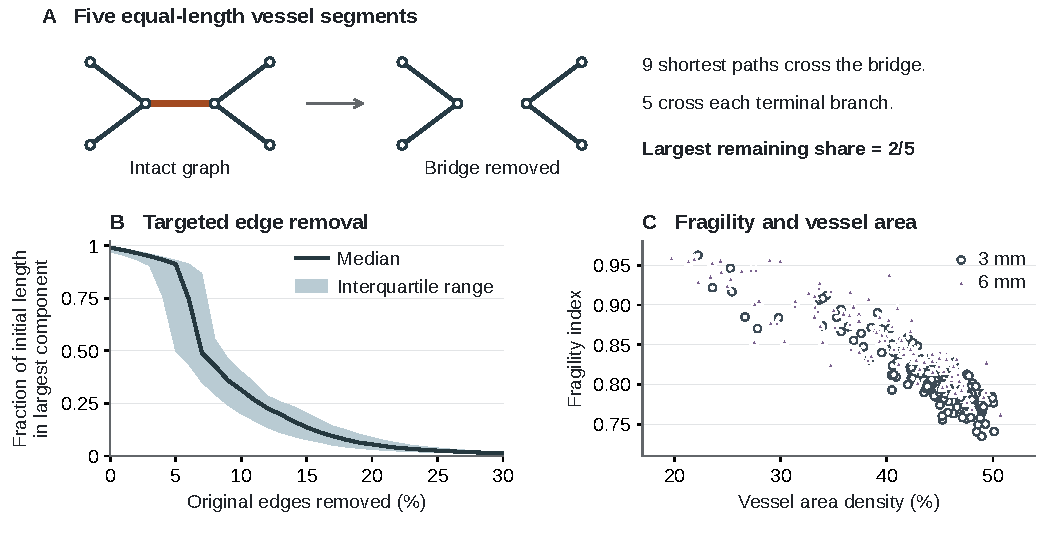
\includegraphics[width=\textwidth]{figures/fragility.pdf}
\caption{Targeted removal of vessel segments. A illustrates the first deletion in a five-segment graph. All segments have unit length. Removing the middle segment leaves two components, each of length two. B shows the median and interquartile range for the first 30\% of deletions in 295 eyes. The curves were interpolated for display. Each eye's index uses its complete deletion sequence. C shows that index against vessel area density for each scan field.}
\label{fig:fragility}
\end{figure*}

\section{Methods}
\subsection{Cohort and Vessel Labels}
OCTA-500 contains macular OCTA scans acquired at Jiangsu Province Hospital from March 2018 to July 2020 with one RTVue-XR system \citep{li2024octa500}. Each participant contributed one eye. The $3\times3$\,mm scans ($304\times304$ pixels) came mainly from healthy participants. A separate recruitment for the $6\times6$\,mm scans ($400\times400$ pixels) drew chiefly from patients with retinal disease. The investigators used the diagnoses recorded by ophthalmologists. The release does not give the clinical criteria for each DR diagnosis, the DR grade, or a separate category for diabetes without retinopathy.

Of 500 eyes, 185 had diagnoses other than DR or normal. A fixed hash of image identifier selected ten healthy eyes per field for calibration. All 295 remaining eligible eyes entered the analysis, including those with poor-quality images (Table~\ref{tab:cohort}). All 295 had complete data for every variable in the primary regression.

\begin{table}[t]
\centering
\small
\begin{tabular}{lrrrr}
\toprule
 & \multicolumn{2}{c}{3 mm} & \multicolumn{2}{c}{6 mm}\\
\cmidrule(lr){2-3}\cmidrule(lr){4-5}
 & Healthy & DR & Healthy & DR\\
\midrule
Eyes & 150 & 29 & 81 & 35\\
Age (years) & 29.9 & 47.3 & 43.8 & 52.6\\
\quad SD & 15.4 & 11.6 & 18.4 & 10.7\\
Male (\%) & 49 & 66 & 58 & 69\\
Vessel length density & 29.0 & 22.5 & 15.2 & 12.5\\
FAZ area (mm$^2$) & 0.33 & 0.52 & 0.34 & 0.46\\
\bottomrule
\end{tabular}
\caption{Analysis cohort by scan field and dataset diagnosis. Age is shown as mean and SD. Length density (mm/mm$^2$) and foveal avascular zone (FAZ) area are group means. Each eye represents a different participant.}
\label{tab:cohort}
\end{table}

The analysis used the maximum-intensity projection from the inner limiting membrane to the outer plexiform layer, which combines several vascular plexuses. The vessel mask was the union of the released capillary and large-vessel masks. The dataset authors generated the capillary labels with a model optimized for topology and manually annotated the large vessels and foveal avascular zone (FAZ) \citep{li2024octa500}. The released vessel labels served as the reference tracing. Density calculations used nominal pixel dimensions without axial-length correction. The analysis area excluded the FAZ and a 50-$\mu$m outer border.

\subsection{Graph Construction and Fragility}
Skeletonization reduced each vessel mask to centerlines. Diagonally adjacent pixels counted as connected only when they shared no horizontal or vertical skeleton neighbor. Clusters of junction pixels formed nodes, degree-one pixels formed endpoints, and intervening paths formed the edges of an undirected multigraph. Edge lengths summed the physical lengths of the pixel steps along each path. Parallel edges and loops were retained. Cleanup removed edges touching the outermost image pixels and edges with at least half their path inside the FAZ. After contracting degree-two nodes, one pruning pass removed terminal spurs shorter than twice the largest neighboring branch width. Components shorter than 50\,$\mu$m were discarded.

\begin{figure*}[t]
\centering
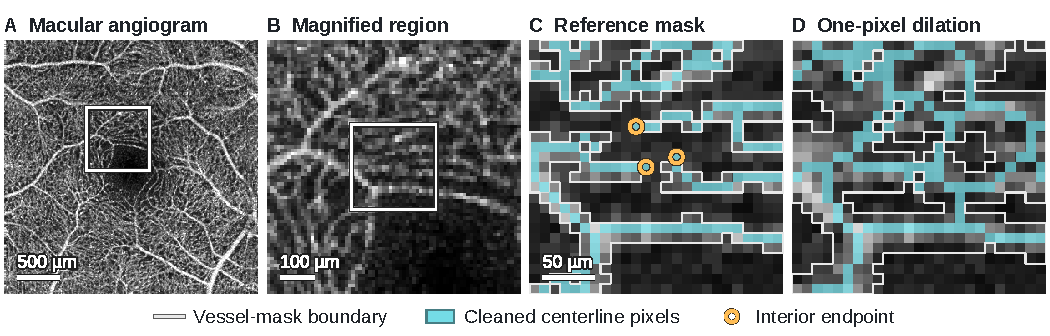
\includegraphics[width=\textwidth]{figures/retinal_tracing.pdf}
\caption{Tracing one retinal angiogram before and after capillary-mask dilation. A shows the first 3-mm scan in the masked review packet. B enlarges the boxed region of A. C and D show the same $25\times25$-pixel window marked in B, selected to illustrate a local gap. Both overlays show the mask boundary and cleaned graph. Within this window, the reference graph has three interior endpoints (C) and the dilated graph has none (D). Degrees were calculated on the full graph before cropping. Image and labels adapted from OCTA-500 (M. Li, S. Yuan and Q. Chen, IEEE DataPort, CC BY 4.0) \citep{li2024octa500}.}
\label{fig:ends}
\end{figure*}

For each edge $e$, the removal algorithm counted how often it lay on a shortest path. Path length was measured along the vessel centerlines. For a connected pair of nodes $u,v$, let $\sigma_{uv}$ be the number of shortest paths and $\sigma_{uv}(e)$ the number that use $e$. The edge's betweenness is
\begin{equation}
 B(e)=\sum_{\{u,v\}}\frac{\sigma_{uv}(e)}{\sigma_{uv}},
 \label{eq:betweenness}
\end{equation}
where the sum covers unordered, connected pairs of distinct nodes. At each step the algorithm deleted the edges with the highest scores and recalculated $B$ on the remaining graph. Each batch contained 1\% of the original edge count, rounded to the nearest integer, with a minimum of one. Edge identifiers broke ties.

The fragility index adapts a measure of network robustness under targeted deletion \citep{schneider2011mitigation}. Let $L_0$ be the total traced length before deletion, $L_k$ the length in the largest connected component after batch $k$, and $K$ the number of batches. Then
\begin{equation}
 F=1-\frac{2}{K}\sum_{k=1}^{K}\frac{L_k}{L_0}.
 \label{eq:fi}
\end{equation}
A larger $F$ means less of the original length stayed connected over the removal sequence. The sum includes the final empty graph. The starting graph may already be disconnected.

In Figure~\ref{fig:fragility}A, nine pairs of nodes connect through the central segment and five through each terminal segment. Deleting the central segment leaves a largest component of length two. Deleting a tip first would leave length four. Recalculating betweenness after each deletion gives successive largest-component lengths of $2,2,1,1,0$. Since $L_0=5$ and $K=5$, the example gives $F=1-2(2+2+1+1+0)/25=0.52$.

\subsection{Comparing Models With and Without Fragility}
The baseline logistic regression estimated the probability of a DR label from scan field, age, sex, vessel area density (the fraction of analysis pixels labeled as vessel), FAZ area, and loop density (independent cycles per mm$^2$). A second regression added graph fragility as its only extra predictor. Both used the same 295 eyes, with DR coded as one and healthy as zero. Continuous predictors were centered on the cohort mean and divided by the sample SD. Indicator variables identified 6-mm scans and male participants.

For eye $i$, let $p_i$ be the modeled probability of DR, $\mathbf{x}_i$ the baseline predictors, and $z(F_i)$ the standardized fragility. The model with fragility was
\begin{equation}
 \log\frac{p_i}{1-p_i}=\alpha+\mathbf{x}_i^{\mathsf T}\boldsymbol{\beta}
                              +\theta z(F_i).
 \label{eq:logit}
\end{equation}
Both models were fitted by unpenalized maximum likelihood. The baseline fixed $\theta=0$. To test whether fragility improved the fit, twice the gain in log likelihood was compared with a $\chi^2$ distribution with one degree of freedom. The adjusted odds ratio for a one-SD increase in fragility was $\exp(\theta)$, with a 95\% Wald confidence interval (CI). Two sensitivity analyses repeated the comparison with fractal dimension replacing loop density or with both measures included.

Discrimination was assessed on held-out eyes. In each of ten repeats, participants were split into five folds stratified by diagnosis. Both predictor sets used the same folds. Ridge logistic regression ($C=1$) was fitted on four folds and predicted DR probabilities in the fifth. Scaling and median imputation used only the training folds. Rotating the held-out fold gave one prediction per eye for each model. The area under the receiver operating characteristic curve (AUROC) was computed from all held-out predictions within each repeat. The reported difference averages the ten paired AUROC differences. A 95\% percentile interval used 2,000 participant samples drawn with replacement within diagnosis groups, keeping each participant's paired predictions together across repeats and the fitted models fixed.

\subsection{Selecting and Counting Endpoints}
An exploratory audit compared ten vessel-derived measurements and FAZ area. Raw endpoint density showed the largest DR--healthy difference after adjustment for field and traced vessel length density. Short spurs and vessels cut off by the edge of the scan can both contribute endpoints. The follow-up analysis counted degree-one nodes on the cleaned graph more than five pixels from both the image edge and the FAZ (about 49\,$\mu$m at 3 mm and 75\,$\mu$m at 6 mm). Figure~\ref{fig:ends} shows how widening the capillary mask can join two nearby paths and change which nodes meet this rule.

For each eye, let $N_i$ be its count of interior endpoints, $A_i$ its analysis area in mm$^2$, and $L_{0i}$ its cleaned vessel length in mm. Endpoint density is $E_i=N_i/A_i$ and vessel length density is $D_i=L_{0i}/A_i$. The unadjusted and adjusted comparisons used the same outcome $Z_i$, obtained by centering $E_i$ on the field mean and dividing by the field SD across both groups. The full comparison was
\begin{equation}
 Z_i=\alpha+\delta\,\mathrm{DR}_i+\gamma\,\mathrm{Wide}_i
             +\lambda D_i+\varepsilon_i,
 \label{eq:end}
\end{equation}
where $\mathrm{DR}_i$ and $\mathrm{Wide}_i$ indicate DR and a 6-mm scan. The coefficient $\delta$ summarizes the DR--healthy difference under the assumption that endpoint density changes at the same rate with traced length density in both groups and scan fields. For the crude comparison we omitted field and length density. A second fit included field alone.

For the eleven-measure audit, each field-standardized measurement in turn was the outcome in Eq.~\ref{eq:end}. The pooled regressions used ordinary least squares, a common length-density slope across groups and fields, and HC3 standard errors. Holm adjustment covered the eleven pooled tests \citep{holm1979simple}. Candidate measures had to pass the adjusted $p<0.05$ threshold, with the same direction and intervals excluding zero in both fields. They also had to retain their association under label perturbations and two image-quality adjustments, and preserve within-field ranks (Spearman $\rho\geq0.80$) under each of three mask perturbations. The random-removal index averaged 100 orders. The coverage measure used the fraction of analysis tissue within 42.4\,$\mu$m of remaining vessels, a distance calibrated in the twenty reserved eyes. FAZ area served as a separately delineated positive control. Its mask stayed fixed during vessel perturbations.

To assess image quality, the full model also included structural optical coherence tomography signal (mean intensity), OCTA vessel-to-background contrast, sharpness (Laplacian variance), and striping (line-to-line variation). Contrast was the difference in mean intensity inside and outside the mask divided by the background SD. Both contrast and endpoint count thus depend on the same tracing. An alternative model used intensity and noise in the FAZ and intensity in large vessels. One analysis restricted each field to the overlap between the groups' observed ranges of contrast and length density, checking each variable separately.

A post hoc check of Eq.~\ref{eq:end} fitted a separate intercept and length-density slope for each diagnosis within each scan field. DR--healthy contrasts were evaluated at the field's 25th and 75th percentiles of length density, pooling diagnoses to define each percentile. A second fit allowed a common natural cubic spline in length density (knots at the field tertiles) and a diagnosis-specific linear slope. To check joint overlap, the quality-adjusted common-slope regression was also refitted using only eyes inside the opposite group's convex hull in length density and contrast within the same field. All these fits used the original field SDs and nominal 95\% HC3 intervals.

Interior endpoints were recounted after three changes to the capillary label. One removed 1\% of pixels at random, one flipped boundary pixels with probability 0.10, and one dilated the label by one pixel with a four-neighbor kernel. The dilation extended the released capillary label by one horizontal or vertical pixel (9.9\,$\mu$m at 3 mm and 15\,$\mu$m at 6 mm). The separate large-vessel label, FAZ, analysis area and interior-endpoint rule stayed fixed. Each condition used its own length density and field SD in Eq.~\ref{eq:end}. To express the effect on the measured count in common units, the paired change was $(N_{i,\mathrm{perturbed}}-N_{i,\mathrm{original}})/A_i$ endpoints per mm$^2$. Median paired changes and median vessel coverage were computed by field. A post hoc regression of the paired change after dilation on diagnosis and original length density used a common slope within each field. It estimates the shift in the DR--healthy contrast with the adjustment variable and outcome units held fixed. The three perturbations were chosen before the interior endpoints were recounted, after the raw endpoint results were known. A post hoc dilation used a common 15\,$\mu$m Euclidean cutoff between pixel centers. This included eight neighboring pixels at 3 mm and four at 6 mm.

\subsection{Alternative Tracings and Graph Quality Review}
The same OCTA images were segmented using an uncalibrated Frangi vesselness filter \citep{frangi1998vesselness}, a capillary-scale Frangi filter, and local adaptive thresholding. For the latter two methods, one parameter per field was varied to match median traced length to the reference on the twenty calibration eyes. A U-Net trained to reproduce the reference masks supplied another tracing on a held-out subset \citep{ronneberger2015unet}. For each tracer the same regression used its own raw endpoint density and its own length density.

The fragility comparison was specified in advance. The planned graph review was still pending, so the analysis was designated exploratory before the disease associations were examined. The subsequent review included 20 eyes, ten per field, selected by a fixed hash without regard to diagnosis. A board-certified retina specialist compared the angiogram with its reference mask and graph overlay. A tracing passed if it mostly followed visible vessels, failed if errors were widespread, and was marked uncertain if the image did not support a judgment. On the same eyes, the specialist rated the two calibrated classical tracers with their identities masked. Diagnoses and analysis results were masked. The specialist had previously seen these eyes in a different layout. The ratings assessed each tracing as a whole. The specialist did not adjudicate individual endpoint locations, and the ratings did not determine eligibility.

A separate experiment used the held-out U-Net to retrace images after blur, additive noise, or dimming, each at three levels. Each original DR or healthy scan was compared with degraded scans from at least three other healthy eyes of the same field within 5\% of its length density. Matching versions were averaged within each donor and then across donors. A participant bootstrap resampled the target eyes with those donor matches held fixed.

\section{Results}
\begin{figure*}[t]
\centering
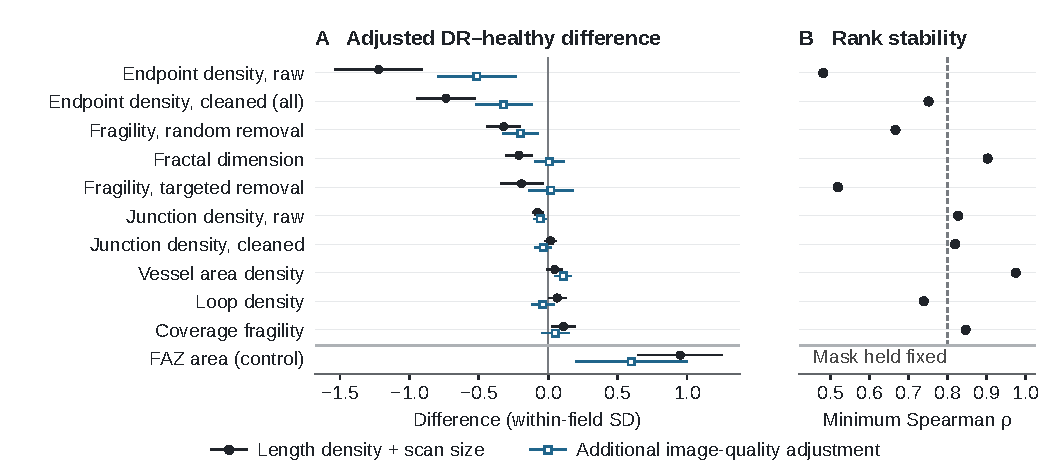
\includegraphics[width=\textwidth]{figures/metric_audit.pdf}
\caption{Differences by diagnosis and sensitivity to mask processing across the eleven audited measures. In A, bars give nominal 95\% HC3 intervals for the DR coefficient (295 eyes). Quality adjustment adds signal, contrast, sharpness, and striping to field and length density. Cleaned endpoint density includes all locations. The interior measure in Table~\ref{tab:pixel} excludes endpoints near the image edge or FAZ. In B, each point gives the lowest within-field rank correlation under dropout, boundary changes, or one-pixel dilation. The dashed line marks the audit threshold. The FAZ mask was held fixed during perturbation.}
\label{fig:audit}
\end{figure*}

\begin{figure*}[t]
\centering
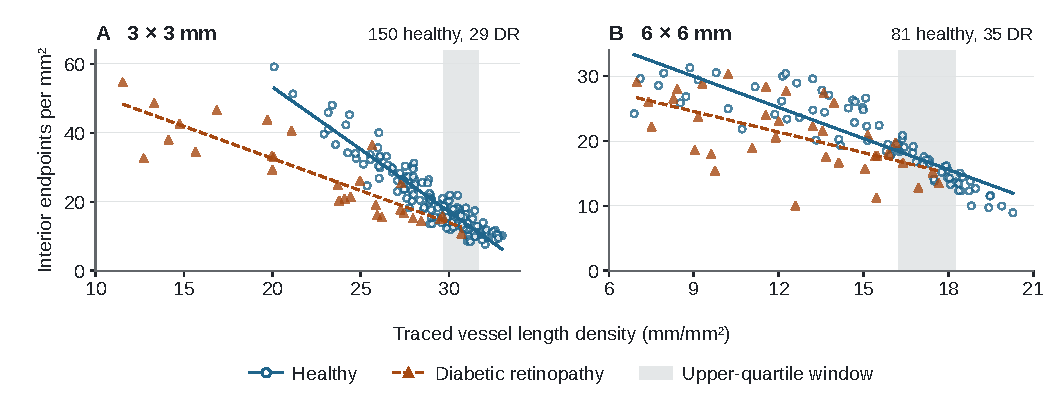
\includegraphics[width=\textwidth]{figures/endpoint_overlap.pdf}
\caption{Interior endpoint density and traced vessel length density on the original masks. Each point is one eye. Lines show separate linear fits by diagnosis over each group's observed range. In each field, the shaded band spans $\pm1$ mm/mm$^2$ around the upper quartile of length density across both groups. Axis ranges differ between fields.}
\label{fig:overlap}
\end{figure*}

\subsection{Fragility Added Little to the Baseline}
The DR group was older and had shorter traced vessel length per unit area in both scan fields (Table~\ref{tab:cohort}). The largest component lost most of its length early in the removal sequence (Figure~\ref{fig:fragility}B). Fragility correlated with vessel area density within each field (Spearman $\rho=-0.85$ at 3 mm and $-0.90$ at 6 mm) and across all 295 eyes ($-0.90$, Figure~\ref{fig:fragility}C). The crude odds ratio for DR per SD of fragility was 2.64 (95\% CI 1.94 to 3.58). With the baseline covariates it was 0.69 (0.25 to 1.93). The log likelihood rose from $-85.552$ to $-85.297$, giving a likelihood-ratio statistic of 0.51 ($p=0.475$). For distinguishing DR cases from healthy controls, the baseline AUROC was 0.901 and the augmented-model AUROC was 0.898 (paired difference $-0.0028$, conditional 95\% CI $-0.0044$ to $-0.0014$).

The coefficient was sensitive to the other topology variable in the model. Substituting fractal dimension for loop density reversed the estimated association (odds ratio 2.56, 95\% Wald CI 0.996 to 6.59, likelihood-ratio $p=0.0499$). Including both fractal dimension and loop density produced fitted probabilities at the boundary and failed the protocol's estimability check. This leaves substantial uncertainty about the adjusted odds ratio despite the small observed change in discrimination.

\begin{table*}[t]
\centering
\begin{tabular}{lcrrrrrr}
\toprule
 & Adjusted DR difference & \multicolumn{2}{c}{Vessel coverage (\%)} & \multicolumn{2}{c}{Change in endpoints/mm$^2$} & \multicolumn{2}{c}{Rank correlation}\\
\cmidrule(lr){3-4}\cmidrule(lr){5-6}\cmidrule(lr){7-8}
Capillary label & SD (95\% CI) & 3 mm & 6 mm & 3 mm & 6 mm & 3 mm & 6 mm\\
\midrule
Original & $-0.74$ ($-0.95$, $-0.53$) & 45.1 & 40.1 & 0.00 & 0.00 & --- & ---\\
1\% dropout & $-0.75$ ($-0.96$, $-0.54$) & 44.7 & 39.8 & $+1.54$ & $+0.76$ & 0.997 & 0.999\\
Boundary flips & $-0.65$ ($-0.87$, $-0.43$) & 45.3 & 40.7 & $+10.10$ & $+2.79$ & 0.969 & 0.988\\
1-pixel dilation & $-0.35$ ($-0.49$, $-0.21$) & 80.8 & 74.1 & $-18.42$ & $-17.69$ & 0.735 & 0.809\\
\bottomrule
\end{tabular}
\caption{Interior endpoints after reprocessing the same 295 eyes. Coverage is the median percentage of analysis pixels labeled as vessel. Change is the median within-eye difference from the original mask. Spearman correlations compare the ranking of these eyes with the original ranking within each field. The pooled DR--healthy coefficient uses each mask's traced length density and within-field outcome SD, with a nominal 95\% HC3 interval.}
\label{tab:pixel}
\end{table*}

\begin{table*}[t]
\centering
\begin{tabular}{lrrccccc}
\toprule
&&&\multicolumn{2}{c}{Length ratio} & & \multicolumn{2}{c}{Graphs passing review}\\
\cmidrule(lr){4-5}\cmidrule(lr){7-8}
Vessel tracing & Eyes & DR eyes & 3 mm & 6 mm & DR difference, SD (95\% CI) & 3 mm & 6 mm\\
\midrule
Reference mask & 295 & 64 & 1.00 & 1.00 & $-1.22$ ($-1.54$, $-0.91$) & 10/10 & 4/10\\
Uncalibrated Frangi & 295 & 64 & 0.10 & 0.11 & $+0.61$ ($+0.41$, $+0.81$) & --- & ---\\
Capillary-scale Frangi & 295 & 64 & 0.76 & 0.74 & $-1.61$ ($-1.94$, $-1.28$) & 10/10 & 5/10\\
Adaptive threshold & 295 & 64 & 1.01 & 0.97 & $-1.14$ ($-1.50$, $-0.78$) & 9/10 & 1/10\\
Held-out U-Net & 77 & 15 & 1.02 & 1.02 & $-1.53$ ($-2.37$, $-0.69$) & --- & ---\\
\bottomrule
\end{tabular}
\caption{Raw endpoint density across vessel tracings. Length ratio is the median ratio of each eye's traced length to its reference length within field. Group differences adjust for field and tracer-specific length density. One masked specialist rated the same ten eyes per field for each of the three tracings with review counts. A dash means the tracing was outside this review packet. The U-Net analysis includes only eyes held out from segmenter training.}
\label{tab:tracer}
\end{table*}

\subsection{Endpoint Density and the Extent of Group Overlap}
After adjustment for length density and field, raw endpoint density had the largest absolute group difference ($-1.22$ SD, 95\% CI $-1.54$ to $-0.91$, Figure~\ref{fig:audit}). It was also the least stable measurement of individual eyes (minimum $\rho=0.48$). None of the ten vessel-derived measurements met all audit criteria. FAZ area, the separately delineated positive control, was larger in DR by 0.95 SD (0.65 to 1.26). At 3 mm, short spurs accounted for much of the raw count. Pruning removed 63\% of raw endpoints in healthy eyes and 50\% in eyes with DR.

On the original cleaned graphs, DR eyes had more interior endpoints per unit area than healthy eyes before adjustment ($+0.40$ SD, 95\% CI $+0.11$ to $+0.69$). Adjusting for field alone gave $+0.41$ SD ($+0.11$ to $+0.71$). Adding length density reversed the sign to $-0.74$ SD ($-0.95$ to $-0.53$) under the common-slope model. These fits used the same 295 eyes, endpoint definition, area denominator and field-specific SD. In healthy eyes, sparser tracings had more endpoints per unit area (Spearman $\rho=-0.93$ at 3 mm and $-0.94$ at 6 mm).

Figure~\ref{fig:overlap} shows where the two groups could be compared. With separate slopes in the 3-mm field, the estimated DR--healthy difference was $-0.89$ SD ($-1.12$ to $-0.66$) at the lower quartile of traced length density and $-0.19$ SD ($-0.53$ to $+0.14$) at the upper quartile. Only one DR eye and 55 healthy eyes fell within 1 mm/mm$^2$ of the upper quartile (30.68 mm/mm$^2$). Allowing curvature, the additional slope for DR relative to healthy eyes was $+0.173$ SD per mm/mm$^2$ ($+0.097$ to $+0.250$) at 3 mm and $+0.012$ ($-0.064$ to $+0.087$) at 6 mm.

For comparison with earlier work that divided counts by vessel length, median interior endpoints per millimeter of traced vessel were also higher in DR before adjustment. The medians were 1.05 versus 0.62 at 3 mm and 1.71 versus 1.21 at 6 mm (DR versus healthy).

Adjustment for signal, contrast, sharpness, and striping gave an interior endpoint difference of $-0.34$ SD ($-0.55$ to $-0.14$). Adding age and sex gave $-0.345$ SD. The field-specific estimates were $-0.45$ SD ($-0.75$ to $-0.15$) at 3 mm and $-0.28$ SD ($-0.57$ to $+0.01$) at 6 mm. The alternative quality proxies yielded a pooled difference of $-0.58$ SD ($-0.80$ to $-0.36$). At 3 mm, contrast in 13 of 29 DR eyes exceeded the highest healthy value. Restriction to the shared range of each variable separately retained 47 DR and 95 healthy eyes (adjusted difference $-0.39$ SD, $-0.59$ to $-0.19$). Requiring joint overlap of length density and contrast retained 35 DR and 69 healthy eyes ($-0.43$ SD, $-0.67$ to $-0.19$).

\subsection{Endpoint Density After Mask Perturbation}
With 1\% dropout, the rank correlation between original and perturbed interior endpoint densities exceeded 0.99 in both fields (Table~\ref{tab:pixel}). Dilation raised median vessel coverage from 45.1\% to 80.8\% at 3 mm and from 40.1\% to 74.1\% at 6 mm. The median within-eye changes in total traced length were $-0.8$\% and $+4.2$\%, respectively. At 3 mm, dilation reordered eyes by interior endpoint density ($\rho=0.735$), even though all ten reference graphs reviewed in this field had passed. The median within-eye loss was 18.42 interior endpoints/mm$^2$ at 3 mm and 17.69 at 6 mm. Holding original length density fixed, the DR--healthy contrast shifted by $+10.98$ endpoints/mm$^2$ ($+7.57$ to $+14.39$) at 3 mm and $+2.77$ ($+1.04$ to $+4.49$) at 6 mm. These estimates use a common slope for the two diagnoses within each field.

With the common 15\,$\mu$m cutoff, median coverage reached 89.4\% at 3 mm and 74.1\% at 6 mm. The rank correlations with the original tracing were 0.606 and 0.809, respectively.

\subsection{Alternative Tracings and Specialist Review}
The uncalibrated Frangi filter traced about one-tenth of the reference vessel length and reversed the raw endpoint difference (Table~\ref{tab:tracer}). After calibration, both classical tracers gave lower endpoint counts in DR at equal modeled length density. The capillary-scale filter produced about three-quarters of the reference length. The adaptive tracer produced approximately the same total length as the reference, yet the specialist passed only one of its ten 6-mm graphs. The U-Net agreed in direction but had learned to reproduce the reference segmentation.

The specialist passed 14 of the 20 reference graphs. Among the ten reviewed at 6 mm, four passed, one failed, and five were uncertain. The failed graph followed a checkerboard artifact. Streaking and grain contributed to uncertain ratings. Only one reviewed 3-mm eye and four reviewed 6-mm eyes had DR. The wider field accounted for 35 of the 64 DR eyes in the study.

In the 62 healthy eyes, median traced length fell and interior endpoints per millimeter rose at the strongest level of each degradation. Severe blur and dimming retained only 6\% and 9\% of original length, respectively (median within-eye ratios). Even the unaltered healthy scans had fewer endpoints per millimeter than their density-matched degraded controls (median difference $-0.12$, 95\% bootstrap CI $-0.15$ to $-0.11$, 59 matched eyes). For the 12 of 15 DR eyes with matches, the median difference was $-0.95$ ($-1.52$ to $-0.50$). Only five of these DR eyes were 6-mm scans. This comparison did not adjust for contrast.

\section{Discussion}
In OCTA-500, fragility closely tracked vessel area density and changed cross-validated AUROC by less than 0.003. Its adjusted odds ratio was imprecise and changed direction when fractal dimension replaced loop density.

On the released tracings, DR eyes had more interior endpoints per unit area as observed. The pooled comparison reversed after adjustment for traced length. The separate fits gave a larger difference in sparser 3-mm tracings. Most eyes with dense tracings were healthy. The negative estimate persisted among eyes with overlapping length density and contrast, although this restriction retained only 104 of 295 eyes. The adjusted estimate compares tracings with similar measured vessel length and holds aside differences in length that may themselves reflect disease. It cannot establish whether DR reduces the number of anatomical vessel endings.

\citet{yu2024branching} found more endpoints per unit vessel length in mild DR in most regions, with little difference in counts. The unadjusted OCTA-500 comparison per unit length followed the same direction. \citet{zare2026remodeling} adjusted for skeleton density and found differences across controls, diabetes without retinopathy, and nonproliferative DR. Their overall test did not identify the direction of the DR--control difference. In three-dimensional reconstructions, \citet{zhang2026radar} found more endpoints in early DR and showed that projection changes the counts. Vessels at different depths can appear to meet on a projection. A vessel can also appear to end where it leaves the imaged slab.

One pixel was enough to join nearby paths in the selected retinal patch (Figure~\ref{fig:ends}). Across the cohort the same operation labeled considerably more tissue as vessel, while total traced length changed little. It provides a stress test of the endpoint measure. How closely this perturbation resembles variation between human tracers or repeat acquisitions is unknown. For medical-image AI that uses vessel graphs as input, a change in segmentation can change which eyes rank highest before a prediction model is fitted. Comparing the same feature across tracing methods can reveal that source of variation. Reporting mask coverage and pixel size puts the stress test in context.

Some sparse healthy tracings may contain short gaps between vessels still visible on either side. A DR tracing of the same total length could contain fewer such gaps. Digital degradation reproduced part of this pattern in healthy eyes, although even unaltered healthy scans differed from their density-matched degraded controls. The experiment cannot establish why a clinical scan was sparse. Image contrast offers only a partial check because it is calculated from the same mask used to count endpoints. Adjusting for contrast may remove disease-related variation along with acquisition effects.

The audit selected the largest of eleven group differences, which can inflate its magnitude. Multiplicity correction covered the eleven tests. The endpoint analyses, including the checks of slope and overlap, reused the discovery eyes. Controls were younger, and the single-device cohort contained only 64 DR eyes. The release includes neither photographic severity grades on the Early Treatment Diabetic Retinopathy Study (ETDRS) scale nor a diabetes-without-retinopathy group. These cross-sectional scans therefore cannot establish progression, a screening threshold, or added value in clinical decisions.

The attempted external test on 12-mm DRAC scans stopped before diagnosis comparisons \citep{qian2024drac}. At native contrast, segmentation followed speckle. Smoothing also removed fine vessels. Clinical validation would require an independent cohort of people with diabetes, including eyes without DR and eyes independently graded across the photographic severity scale \citep{etdrs1991grading}. Anatomical validation poses a different question. Masked readers could independently mark endpoint locations on registered, depth-resolved repeat scans of the same eye and assess whether an apparent ending recurs, continues in an adjacent slab, or falls at a gap in signal. The present whole-graph ratings cannot resolve those alternatives.

\section{Data Availability and Disclosures}
\noindent\textbf{Data availability.} IEEE DataPort distributes the OCTA-500 scans and labels \citep{li2024octa500}. The analysis code, figure inputs and manuscript are available at \mbox{\pdfstartlink attr {/Border [0 0 0]} user {/Subtype /Link /A << /S /URI /URI (https://github.com/kameronlee/dr-analysis) >>}\url{https://github.com/kameronlee/dr-analysis}\pdfendlink}. 

\begin{samepage}\noindent\textbf{Funding.} This secondary analysis received no funding and used George Mason University's Hopper cluster. OCTA-500 received support from the National Natural Science \mbox{Foundation of China} and the Fundamental Research Funds for the Central Universities \citep{li2024octa500}.\par\end{samepage}

\noindent\textbf{Competing interests.} The retina specialist who reviewed the tracings is a family member of the author.

\bibliography{references}
\end{document}
